\documentclass[11pt, oneside]{article} 
\usepackage{geometry}
\geometry{letterpaper} 
\usepackage{graphicx}
	
\usepackage{amssymb}
\usepackage{amsmath}
\usepackage{parskip}
\usepackage{color}
\usepackage{hyperref}

\graphicspath{{/Users/telliott/Github/figures/}}
% \begin{center} \includegraphics [scale=0.4] {gauss3.png} \end{center}

\title{Sum of angles}
\date{}

\begin{document}
\maketitle
\Large

%[my-super-duper-separator]

\label{sec:sum_angles_similar_tri}

\subsection*{cosine of a sum}

The sum of angle formulas (formulas for the sine and cosine of the sum or difference of two angles) are used often in calculus, not only for working problems, but even in finding an expression for the derivative of sine and cosine.

You really must know them.  I think it's so important that we will show three ways of finding these formulas.  The easiest way to remember them uses Euler's equation.  We'll see that at the end of the chapter.

There are four equations.  One each for $\sin s \pm t$ and $\cos s \pm t$.

I've memorized only this one:
\[ \cos s - t = \cos s \cos t + \sin s \sin t \]

By $\cos s - t$ we mean $\cos (s - t)$, but have left off the parentheses.  Say "cos cos" and then recall the difference in sign.

\subsection*{check}

I like this version because it can be checked easily.  Just set $s = t$:
\[ \cos s - t = \cos 0 = 1 = \cos^2 s + \sin^2 s \]
which is our favorite trigonometric identity and obviously correct.

As another check we can ask what happens to the formula 
\[ \cos s + t = \cos s \cos t - \sin s \sin t \]
when $t = 0$.  Then the first term is the cosine of $s$, and the second term is equal to $0$.  The formula is symmetrical with respect to $s$ and $t$.

\subsection*{change signs}

For $\cos s + t $ flip the sign on the second term.  
\[ \cos s + t = \cos s \cos t - \sin s \sin t \]
That's because
\[ \cos -\theta = \cos \theta \]
\[ \sin - \theta = - \sin \theta \]

\begin{center} 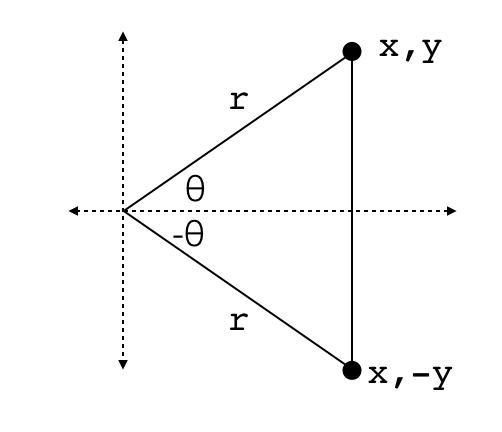
\includegraphics [scale=0.4] {pm_theta.png} \end{center}

The diagram shows the reason:
\[ \cos \theta = \cos - \theta = x/r \]
while
\[ \sin \theta = y/r = -  (\sin - \theta ) = - (-y/r) \]

\emph{Proof}.

Substitute $- \sin \theta$ for $\sin - \theta$ and $\cos \theta$ for $\cos - \theta$:
\[ \cos s - t = \cos s \cos - t + \sin s \sin - t \]
\[ = \cos s \cos t - \sin s \sin t \]

\subsection*{sine of a sum}
We will look at the proof for the sine formula later, for now just write it:
\[ \sin s + t = \sin s \cos t + \sin t \cos s \]

Say "sin cos" and then, that here $+$ goes with $+$.  Like most things having to do with sine and cosine, there is a change of sign when moving from one to the other.

For $\sin s - t$, change the sign on the second term, as before.

Here is a geometric derivation of both of the sum of angles formulas, using similar triangles.  The key is to draw an inspired diagram.

\emph{Proof}.

Consider a right triangle, with one of the angles labeled $s$.  Construct another right triangle containing angle $t$, and scale it so that the base adjacent to angle $t$ is the hypotenuse of the triangle containing angle $s$, drawing them one on top of the other as shown:

Scale the combined triangles so that the hypotenuse of the second triangle has unit length.
\begin{center} \includegraphics [scale=0.4] {sum_angles_3.png} \end{center}

Our crucial insight is to draw vertical and horizontal dotted lines as shown, and to recognize that the small triangle near the top has angle $s$ because its complement is $t + \phi$.  

We add some labels to the sides of the triangles.
\begin{center} \includegraphics [scale=0.4] {sum_angles_4.png} \end{center}

In the left panel, the first two labels are easy:  $\sin t$ and $\cos t$.

For the next part, we need to remember something.  The sine and cosine are ratios of side lengths.  If the hypotenuse is equal to $1$, as for the triangle with angle $t$, then the side \emph{is} the sine or cosine.  But if the hypotenuse is some other value, like $\cos t$, then the side in question, divided by $\cos t$, gives the correct value.  

This explains why the sides of the triangle with angle $s$ on the bottom are labeled as $\cos s \cos t$ and $\sin s \cos t$.  When divided by $\cos t$, they give the correct result for the ratio.  The other two red labels in the right panel are explained in the same way.

Now we simply have to look for $\cos s + t$ and $\sin s + t$ in the figure.  I claim that
\[ \cos s + t + \sin s \sin t = \cos s \cos t \]
and 
\[ \sin s \cos t + \cos s \sin t = \sin s + t \]

$\square$

\subsection*{alternative derivation}
I want to show a short computation that gives the same result as we obtained above. 

The first uses Euler's formula:
\[ e^{ix} = \cos x + i \sin x \]
If you've never seen it before, don't worry.  Just treat $i$ as a constant with $i^2 = -1$.  So then
\[ (\cos s + i \sin s)(\cos t + i \sin t) \]
\[ = \cos s \cos t - \sin s \sin t + i \ [ \ \sin s \cos t + \cos s \sin t \ ] \] 
This is an \emph{imaginary} number with a real part (the first two terms), plus an imaginary part, with the leading $i$.

In terms of the exponential
\[ e^{is} \cdot e^{it} = e^{i(s+t)} \]
\[ = \cos s + t + i \sin s + t \]

By Euler's formula, these two expressions are equal.  The rule is that both the real parts and the imaginary parts must be equal.  So we have
\[ \cos s + t = \cos s \cos t - \sin s \sin t \]
\[ \sin s + t = \sin s \cos t + \cos s \sin t \]

There is another easy derivation based on the idea of rotation of unit vectors.  But you need to understand a bit about matrix multiplication for that.  Basically the idea is that a point $x,y$ in the plane can be represented as a vector:
\[ 
\begin{bmatrix}
x \\
y
\end{bmatrix}
\]
Rotation of the vector amounts to multiplication by a matrix
\[
\begin{bmatrix}  
\cos \theta & -\sin \theta \\
\sin \theta & \ \  \cos \theta 
\end{bmatrix}
\begin{bmatrix}  x \\ y \end{bmatrix}
=
\begin{bmatrix}  u \\ v \end{bmatrix}
\]
Rotation by angle $\theta + \phi$ is the same as rotation first by angle $\theta$ and then by angle $\phi$ so
\[
\begin{bmatrix}  
\cos \theta & -\sin \theta \\
\sin \theta & \ \  \cos \theta 
\end{bmatrix}
\begin{bmatrix}  
\cos \phi & -\sin \phi \\
\sin \phi & \ \  \cos \phi 
\end{bmatrix}
=
\begin{bmatrix}  
\cos \theta + \phi & -\sin \theta + \phi \\
\sin \theta + \phi & \ \  \cos \theta + \phi
\end{bmatrix}
\]
The rule for matrix multiplication quickly gives our two formulas.

\subsection*{double-angle formulas}
Very quickly, sine:
\[ \sin s + t = \sin s \cos t + \cos s \sin t \]
\[ \sin 2t = 2 \sin t \cos t \]
And cosine:
\[ \cos s + t = \cos s \cos t - \sin s \sin t \]
\[ \cos 2t = \cos^2 t - \sin^2 t = 2 \cos^2 t - 1 \]

\subsection*{another calculation}
We found previously that 
\[ \sin \frac{\pi}{4} = \cos \frac{\pi}{4} = \frac{1}{\sqrt{2}} \]
\[ \sin \frac{\pi}{6} = \cos \frac{\pi}{3} = \frac{1}{2}; \ \ \ \ \sin \frac{\pi}{3} = \cos \frac{\pi}{6} = \frac{\sqrt{3}}{2} \]

These angles correspond to 30, 45 and 60 degrees.  It might be nice to have sine and cosine of 15 and 75 degrees as well.  That would make even divisions of the first 90 degrees.  We can get them as the sum and difference of $\pi/4$ and $\pi/6$.

Let $s = \pi/4$ and $t = \pi/6$.  Then

\[ \sin \frac{\pi}{12} = \sin s - t = \sin s \cos t - \sin t \cos s \]
\[ = \frac{1}{\sqrt{2}} \cdot \frac{\sqrt{3}}{2} - \frac{1}{2} \cdot \frac{1}{\sqrt{2}} = \frac{\sqrt{3} - 1}{2 \sqrt{2}} \]
\[ \cos \frac{\pi}{12} = \cos s - t = \cos s \cos t + \sin s \sin t \]
\[ = \frac{\sqrt{3}}{2} \cdot \frac{1}{\sqrt{2}} - \frac{1}{2} \cdot \frac{1}{\sqrt{2}} = \frac{\sqrt{3} + 1}{2 \sqrt{2}} \]

We just check that $\sin^2 \theta + \cos^2 \theta = 1$:
\[ \frac{(\sqrt{3} - 1)^2 + (\sqrt{3} + 1)^2}{(2 \sqrt{2})^2} \]
\[ = \frac{3 - 2 \sqrt{3} + 1 + 3 + 2 \sqrt{3} + 1}{8} = 1 \]

We can calculate similarly for $s + t = 5 \pi/12$ or just switch sine and cosine from $\pi/12$.

\end{document}